\documentclass[a4paper,11pt]{article}
\usepackage[utf8]{inputenc}
\usepackage[english]{babel} % Adds processing for some simple special characters.

% Packages for better page formatting and nice footnotes. %
\usepackage{fancyhdr} % Headers.
\usepackage{multicol} % Columns.
\usepackage[margin=0.75in]{geometry} % Margins.
\pagestyle{fancy}
\fancyhf{} % What does this do?
\lhead{Alexander S. Wheaton}
\rhead{\today}
\cfoot{\thepage}

% Title and author for title page. %

\title{AGN Host Properties}
\author{
    Alexander S. Wheaton\\
    School of Physics and Astronomy\\
    The University of Edinburgh\\
    s1572046@ed.ac.uk\break
}

% Utilities for fine-grained control over image insertion. %

\usepackage{graphicx} % Insert images.
\usepackage{float} % Images float in document environment.
\usepackage{wrapfig} % Image/tables in multicols with \wrapfigure or \wraptable.
\usepackage{caption} % Captions for single images.
\usepackage{subcaption} % Captions for simultaneous images.
\graphicspath{ {./img/} }

% Not sure what this is for. %

\usepackage{fullpage,epsf}
\usepackage{lipsum}

% Some utilities for scientific and mathematical writing. %

\usepackage{siunitx} % Formatting for numbers with SI units.
\usepackage{amsmath} % Nice matrices.
% \usepackage{mathabx} % Astronomical symbols.
\usepackage{isotope} % Nice markup syntax for chemical symbols.
\usepackage{xfrac}   % Slant fractions and other utilities.

% Utilities for manual kerning adjustment. %

\newcommand\K{\kern.05em} % Small amount of kerning.
\newcommand\KK{\kern.1em} % Medium amount of kerning.
\newcommand\KKK{\kern.2em} % Large amount of kerning.
\newcommand\KKKK{\kern.3em} % Very large amount of kerning.

% Bibliography and referencing style. Use style=draft for troubleshooting.
\usepackage[backend=bibtex,style=phys,sorting=nyt]{biblatex}
\addbibresource{references.bib}

% Page formatting.

\begin{document}

\thispagestyle{empty}                   % No numbers of title page
\epsfxsize=40mm                         % Size of crest
\begin{minipage}[b]{110mm}
    {\Huge\bf School of Physics\\ and Astronomy
    \vspace*{17mm}}
\end{minipage}
\hfill
\begin{minipage}[t]{40mm}
    \makebox[40mm]{
    
\includegraphics[width=40mm]{crest.eps}}
\end{minipage}
\par\noindent                                           % Centre Title, and name
\vspace*{2cm}
\begin{center}
    \Large\bf \Large\bf MPhys Project\\
    \Large\bf Astrophysics\\[10pt]                     % Change to MP/CP/Astro
    \LARGE\bf Bayesian Inference of Star Formation History in the Host Galaxies of Tidal Disruption Events
\end{center}
\vspace*{0.5cm}
\begin{center}
    \bf Alexander S. Wheaton\\
    \today
\end{center}
\vspace*{5mm}

\begin{abstract}
    \lipsum[1]
\end{abstract}

\vspace*{1cm}

\subsubsection*{Declaration}
\begin{quotation}
    I declare that this project and report is my own work.
\end{quotation}

\hspace*{1cm}Signature:\hspace*{1cm}\includegraphics[width=6cm]{signature_repaired.eps}\hspace*{1cm}Date: \today

\vfill
\noindent{\bf Supervisor:} Professor A. Lawrence, FRSE, FRaS
\hfill
22 Weeks

\newpage
\setcounter{page}{1} % Set page number to 1
\tableofcontents

\newpage
\section{Introduction}\label{sec:introduction}
\subsection{Galaxy Evolution}
compared to stellar Evolution

star formation - black hole mass relation Vieullex 2008
\subsection{Motivation: The AGN-Starburst Connection}\label{sec:agn_starburst_connection}
andy review

\subsection{Evolution of Post-TDE Galaxies}

\subsection{Stellar Population Fitting}\label{sec:stellar_population_fitting}

\section{Fitting with Bagpipes}\label{sec:fitting_with_bagpipes}

The parameter space minimally covered is:

\begin{itemize}
  \item functional form of the SFH
  \item host galaxy redshift
  \item velocity dispersion
  \item dust attenuation curve
\end{itemize}

\section{The XSHOOTER Data}\label{sec:xshooter_data}

\begin{tabular}{| l | c | c | c | c | c | r |}
  \hline
  TDE         & Host Galaxy               & $\alpha$     & $\delta$     & $m$ & Morphology & z        \\
  \hline
  ASASSN-14li & ASASSN-14li               & 12:48:15.23  & +17:46:26.44 & 15  & S3         & 0.0206   \\
  ASASSN-15oi & ASASSN-15oi               & 20:39:09.18  & -30:45:20.10 & 16  & S3         & 0.0484   \\
  AT2018fyk   & LCRS B224721.6-450748     & 22:50:16.090 & -44:51:53.50 & 17  & SBc        & 0.06     \\
  AT2019ahk   & WISEA J070011.40-660224.7 & 07:00:11.546 & -66:02:24.14 & 17  & SBc        & 0.026211 \\
  AT2019azh   & KUG 0810+227              & 08:13:16.945 & +22:38:54.03 & 15  & SBc        & 0.022    \\
  AT2019dsg   & WISEA J205702.96+141216.2 & 20:57:02.974 & +14:12:15.86 & 15  & E7         & 0.0512   \\
  AT2019qiz   & WISEA J044637.88-101334.9 & 04:46:37.880 & -10:13:34.90 & 15  & S0         & 0.01513  \\
  iPTF16fnl   & iPTF16fnl                 & 00:29:57.010 & +32:53:37.24 & 16  & E6         & 0.018    \\
  % AT2018hyz   & WISEA J100650.83+014133.4 & 10:06:50.871 & +01:41:34.08 & 17  &          & 0.04573  \\
  % ASASSN-14ae & ASASSN-14ae               & 11:08:40.12  & +34:05:52.23 & 17  &          & 0.0436   \\
  \hline
\end{tabular}

\section{Blind Testing}\label{sec:blind_testing}

\subsection{Selecting Physically Reasonable Priors}\label{sec:prior_selection}

Velocity dispersion of constituent stars is allowed to vary between

The ionization parameter for nebular emission is allowed to vary between logU=-4 and logU=-2, a very low and very high rate of (molecular?) ionization.

The lifetime of the stellar birth clouds was chosen to be a normal distribution about ${t_{BC}=17Myr}$ with ${\sigma=4Myr}$, consistent with typical cloud lifetimes in the Milky Way, as determined by Murray 2011\cite{Murray_2011}.

\subsection{Run No. 1 (R1): Bulk Formation with Optional Burst}

For my first fitting run, I tried to first establish the functional form of the
old, bulk star formation, and then determine whether or not a more recent burst
improved the fit. I first fit each of the following functions:

\begin{tabular}{| c | c |}
  \hline
  \multicolumn{2}{| c |}{$SFR=e^{t/\tau}$} \\
  \hline
  $t$ & (3.5, 10.0) \\
  $\tau$ & (0.1, 2.0) \\
  $\log_{10}(\sfrac{M}{M_\odot})$ & (0.0, 15.0) \\
  $\sfrac{Z}{Z_\odot}$ & (0.0, 2.5) \\
  \hline
\end{tabular}

\begin{tabular}{| c | c |}
  \hline
  \multicolumn{2}{| c |}{$SFR=te^{\sfrac{-t}{\tau}}$} \\
  \hline
  $t$ & (3.5, 10.0) \\
  $\tau$ & (0.1, 2.0) \\
  $\log_{10}(\sfrac{M}{M_\odot})$ & (0.0, 15.0) \\
  $\sfrac{Z}{Z_\odot}$ & (0.0, 2.5) \\
  \hline
\end{tabular}

\begin{tabular}{| c | c |}
  \hline
  \multicolumn{2}{| c |}{$SFR=lognormal$} \\
  \hline
  $t_{max}$ & (3.5, 10.5) \\
  $2\sigma$ & (0.1, 5.0) \\
  $\log_{10}(\sfrac{M}{M_\odot})$ & (0.0, 15.0) \\
  $\sfrac{Z}{Z_\odot}$ & (0.0, 2.5) \\
  \hline
\end{tabular}

\begin{tabular}{| c | c |}
  \hline
  \multicolumn{2}{| c |}{Global Priors} \\
  \hline
  Dust Type & Calzetti \\
  $A_V$ & (0.0, 1.0) \\
  $z$ & (0.0, 0.1) \\
  $T_{bc}$ & (0.005, 0.015) \\
  $\sigma_{v}$ & (150.0, 200.0) \\
  \hline
\end{tabular}

Once the best-fit functional form of the old, bulk star formation is determined, a new fit is run with that form in linear combination with a delta function, with priors:

\begin{tabular}{| c | c |}
  \hline
  \multicolumn{2}{| c |}{$SFR=\delta_a(t)$} \\
  \hline
  $a$ & (0.1, $a_{low}$) \\
  $\log_{10}(\sfrac{M}{M_\odot})$ & (0.0, 15.0) \\
  $\sfrac{Z}{Z_\odot}$ & (0.0, 2.5) \\
  \hline
\end{tabular}

\subsection{Run No. 2 (R2): Bulk Formation with Burst over Wide Parameter Space}

One of the three functional forms above \textit{or} the more versatile double power law function:

\begin{equation}
  \mathrm{SFR}(t) \propto \left[ \left(\frac{t}{\tau}\right)^{\alpha} + \left(\frac{t}{\tau}\right)^{-\beta} \right]^{-1}
\end{equation}

With priors:

\begin{tabular}{| c | c |}
  \hline
  \multicolumn{2}{| c |}{$\mathrm{SFR}(t)\propto\left[\left(\sfrac{t}{\tau}\right)^{\alpha}+\left(\sfrac{t}{\tau}\right)^{-\beta} \right]^{-1}$} \\
  \hline
  $\tau$ & (0.0, 15.0) \\
  $\alpha$ & (0.0, 10.0) \\
  $\beta$ & (0.0, 10.0) \\
  $\log_{10}(\sfrac{M}{M_\odot})$ & (0.0, 15.0) \\
  $\sfrac{Z}{Z_\odot}$ & (0.0, 2.5) \\
  \hline
\end{tabular}

And with an exponentially decaying burst, the age of which is allowed to vary over a much larger parameter space:

\begin{tabular}{| c | c |}
  \hline
  \multicolumn{2}{| c |}{$SFR=e^{t/\tau}$} \\
  \hline
  $t$ & (0.0, 10.0) \\
  $\tau$ & (0.1, 2.0) \\
  $\log_{10}(\sfrac{M}{M_\odot})$ & (0.0, 15.0) \\
  $\sfrac{Z}{Z_\odot}$ & (0.0, 2.5) \\
  \hline
\end{tabular}

\subsection{Run No. 3 (R3): Bulk Formation with Burst, z-constrained}



\subsection{Run No. 4 (R4): Quenching at Cosmic Noon}

\begin{tabular}{| c | c |}
  \hline
  \multicolumn{2}{| c |}{$SFR=e^{t/\tau}$} \\
  \hline
  $t$ & (7.5, 12.5) \\
  $\tau$ & (0.5, 2.0) \\
  $\log_{10}(\sfrac{M}{M_\odot})$ & (5.0, 12.5) \\
  $\sfrac{Z}{Z_\odot}$ & (0.0, 2.5) \\
  \hline
\end{tabular}

\begin{tabular}{| c | c |}
  \hline
  \multicolumn{2}{| c |}{$SFR=te^{\sfrac{-t}{\tau}}$} \\
  \hline
  $t$ & (7.5, 12.5) \\
  $\tau$ & (0.1, 2.0) \\
  $\log_{10}(\sfrac{M}{M_\odot})$ & (5.0, 12.5) \\
  $\sfrac{Z}{Z_\odot}$ & (0.0, 2.5) \\
  \hline
\end{tabular}

\begin{tabular}{| c | c |}
  \hline
  \multicolumn{2}{| c |}{$SFR=lognormal$} \\
  \hline
  $t_{max}$ & (1.0, 6.0) \\
  $2\sigma$ & (0.1, 3.0) \\
  $\log_{10}(\sfrac{M}{M_\odot})$ & (5.0, 12.5) \\
  $\sfrac{Z}{Z_\odot}$ & (0.0, 2.5) \\
  \hline
\end{tabular}

\begin{tabular}{| c | c |}
  \hline
  \multicolumn{2}{| c |}{$\mathrm{SFR}(t)\propto\left[\left(\sfrac{t}{\tau}\right)^{\alpha}+\left(\sfrac{t}{\tau}\right)^{-\beta} \right]^{-1}$} \\
  \hline
  $\tau$ & (0.0, 4.5) \\
  $\alpha$ & (5.0, 10.0) \\
  $\beta$ & (5.0, 10.0) \\
  $\log_{10}(\sfrac{M}{M_\odot})$ & (5.0, 12.5) \\
  $\sfrac{Z}{Z_\odot}$ & (0.0, 2.5) \\
  \hline
\end{tabular}

And an exponentially declining burst with priors:

\begin{tabular}{| c | c |}
  \hline
  \multicolumn{2}{| c |}{$SFR=e^{t/\tau}$} \\
  \hline
  $t$ & (0.0, 3.5) \\ %Gyr, lifetime of F type stars
  $\tau$ & (0.1, 2.0) \\
  $\log_{10}(\sfrac{M}{M_\odot})$ & (0.0, 12.5) \\
  $\sfrac{Z}{Z_\odot}$ & (0.0, 2.5) \\
  \hline
\end{tabular}

\begin{tabular}{| c | c |}
  \hline
  \multicolumn{2}{| c |}{Global Priors} \\
  \hline
  Dust Type & Calzetti \\
  $z$ & ($z_{obs}-0.001$, $z_{obs}+0.001$) \\ % z varies tight_layout around z_obs.
  $\sigma_{v}$ & (50.0, 450.0) \\ % Constrained by Faber-Jackson. TODO: Lookup Minkowski 1962!
  $T_{bc}$ & (0.013, 0.021) \\  % Constraints from Murray 2011.
  $A_V$ & (0.0, 2.0) \\
  $\log{U}$ & (-4.0, -2.0) \\
  \hline
\end{tabular}

\subsection{Results}\label{sec:results}

\begin{figure}[h!]
\centering
  \includegraphics[width=0.9\textwidth]{../pipes/plots/priors/phil_model_01_sfh.pdf}
  \includegraphics[width=0.9\textwidth]{../pipes/plots/lognormal_noburst/phil_model_01_sfh.pdf}
  \includegraphics[width=0.9\textwidth]{../pipes/plots/wide_lognormal_burst/phil_model_01_sfh.pdf}
  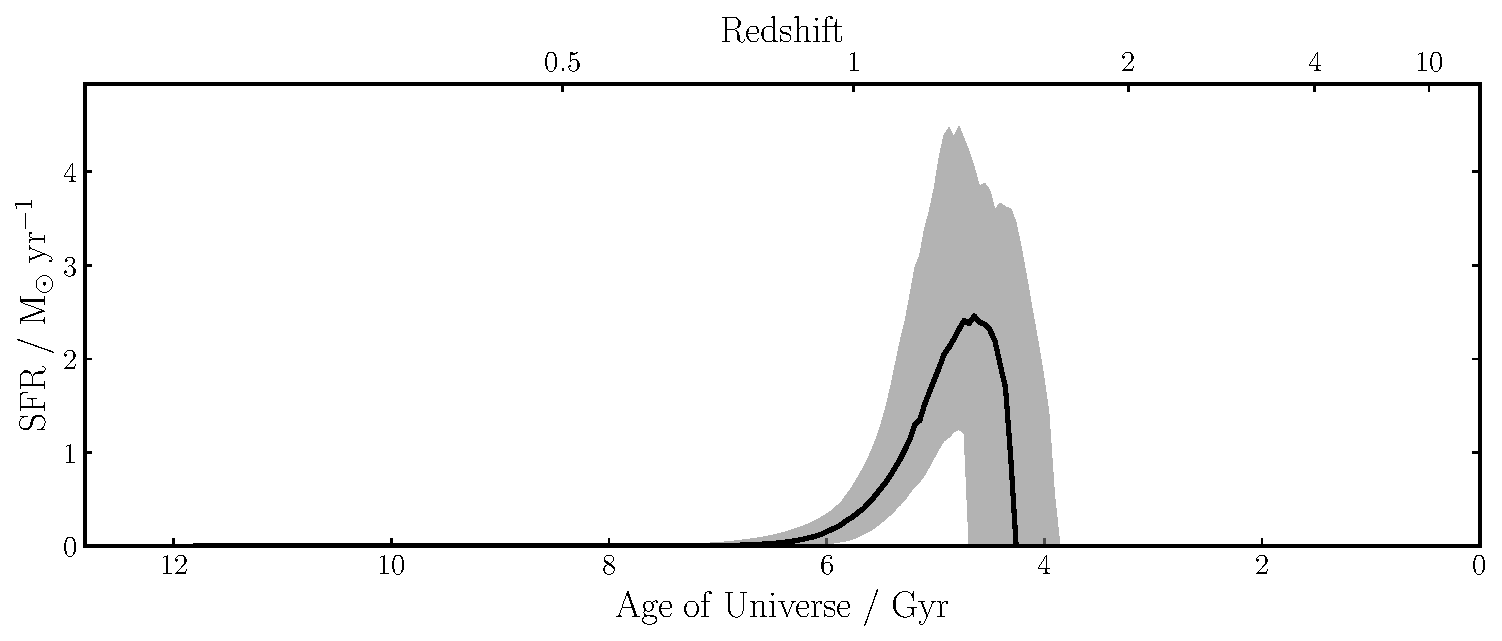
\includegraphics[width=0.9\textwidth]{../pipes/plots/lognormal_burst_final/phil_model_1_sfh.pdf}
  \caption{A priori and posterior SFH.}
  \label{}
\end{figure}

\newpage
\begin{figure}[h!]
  \centering
  \includegraphics[width=0.9\textwidth]{../pipes/plots/priors/phil_model_02_sfh.pdf}
  \includegraphics[width=0.9\textwidth]{../pipes/plots/exponential_burst/phil_model_02_sfh.pdf}
  \includegraphics[width=0.9\textwidth]{../pipes/plots/wide_dblplaw_burst/phil_model_02_sfh.pdf}
  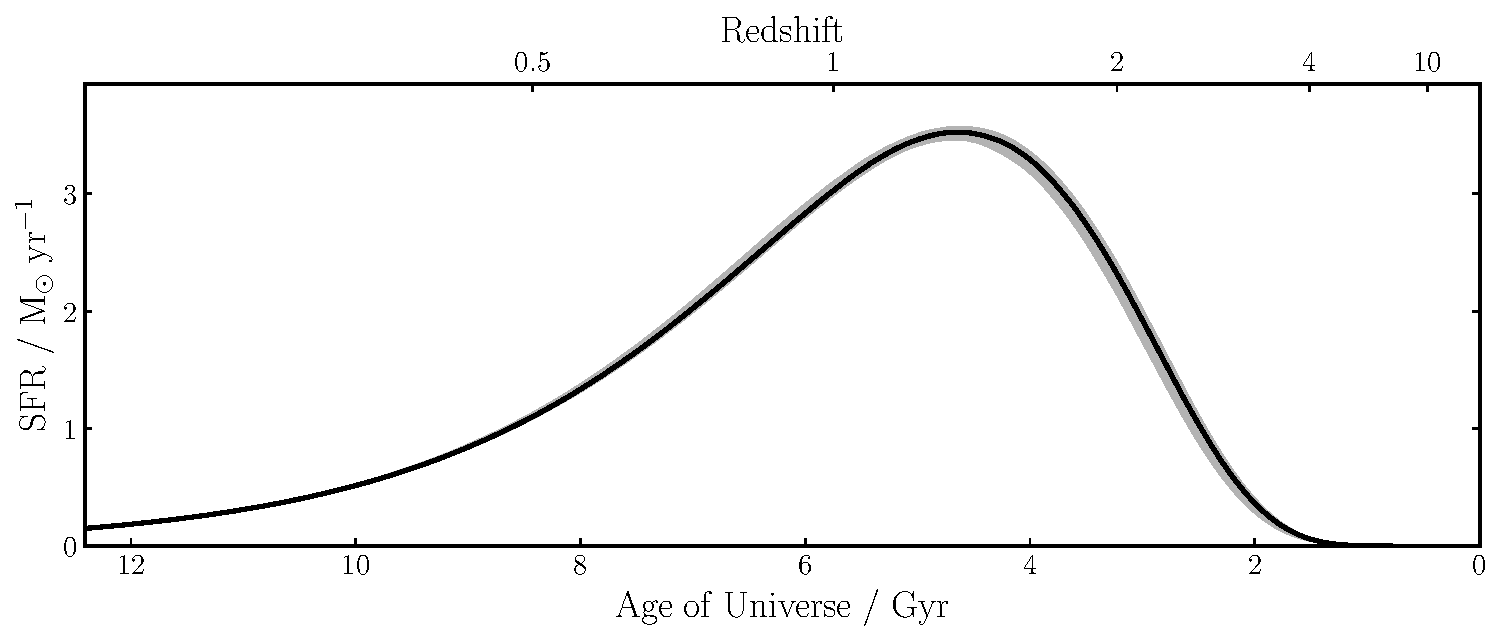
\includegraphics[width=0.9\textwidth]{../pipes/plots/exponential_burst_final/phil_model_2_sfh.pdf}
  \caption{A priori and posterior SFH.}
  \label{}
\end{figure}

\newpage
\begin{figure}[h!]
  \centering
  \includegraphics[width=0.9\textwidth]{../pipes/plots/priors/phil_model_03_sfh.pdf}
  \includegraphics[width=0.9\textwidth]{../pipes/plots/delayed_burst/phil_model_03_sfh.pdf}
  \includegraphics[width=0.9\textwidth]{../pipes/plots/wide_delayed_burst/phil_model_03_sfh.pdf}
  \caption{A priori and posterior SFH.}
  \label{}
\end{figure}

\newpage
\begin{figure}[h!]
  \centering
  \includegraphics[width=0.9\textwidth]{../pipes/plots/priors/phil_model_04_sfh.pdf}
  \includegraphics[width=0.9\textwidth]{../pipes/plots/lognormal_burst/phil_model_04_sfh.pdf}
  \includegraphics[width=0.9\textwidth]{../pipes/plots/wide_lognormal_burst/phil_model_04_sfh.pdf}
  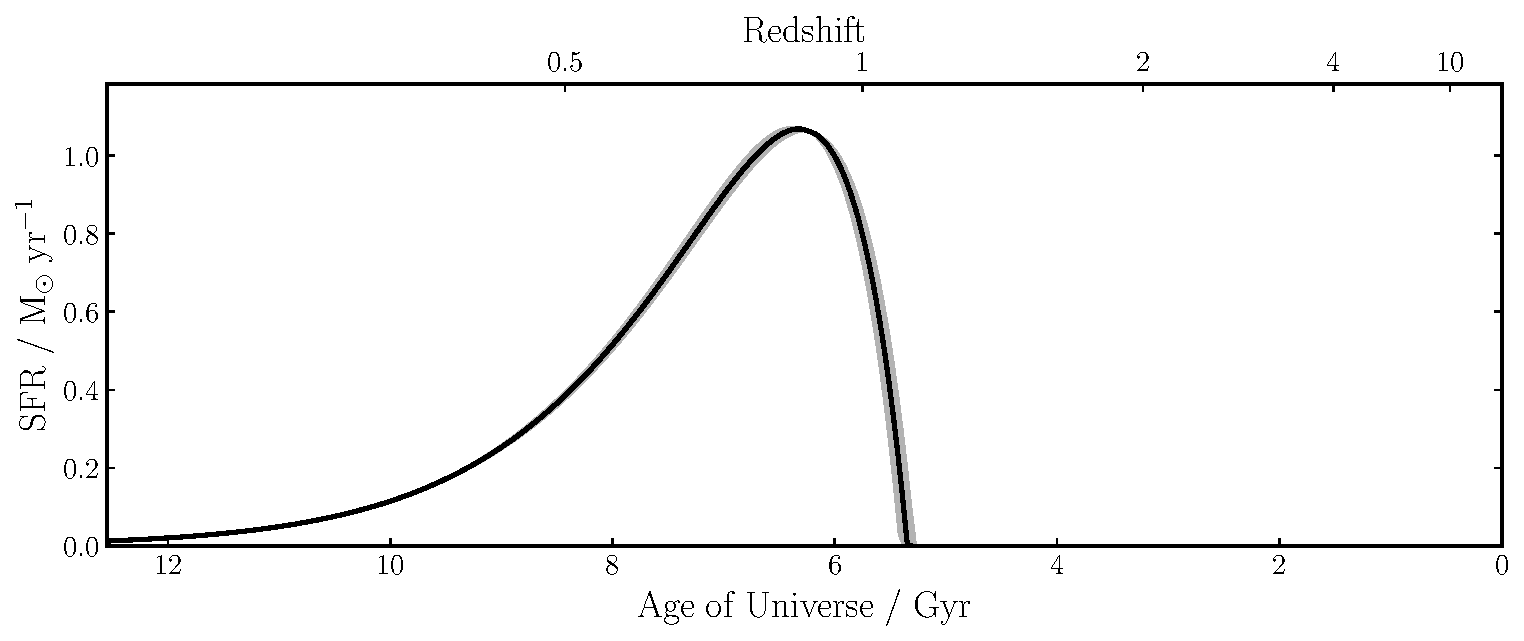
\includegraphics[width=0.9\textwidth]{../pipes/plots/exponential_burst_final/phil_model_4_sfh.pdf}
  \caption{A priori and posterior SFH.}
  \label{}
\end{figure}

\newpage
\begin{figure}[h!]
  \centering
  \includegraphics[width=0.9\textwidth]{../pipes/plots/priors/phil_model_05_sfh.pdf}
  \includegraphics[width=0.9\textwidth]{../pipes/plots/exponential_noburst/phil_model_05_sfh.pdf}
  \includegraphics[width=0.9\textwidth]{../pipes/plots/exponential_noburst/phil_model_05_sfh.pdf}
  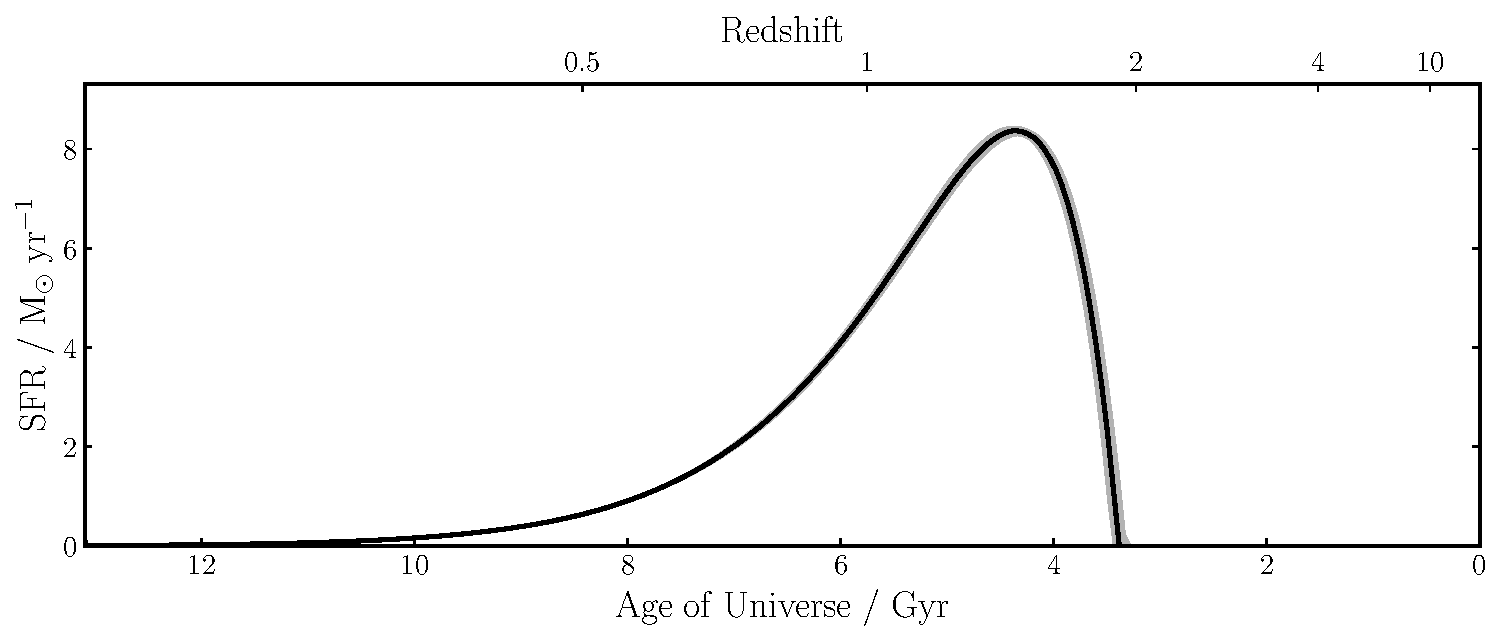
\includegraphics[width=0.9\textwidth]{../pipes/plots/delayed_burst_final/phil_model_5_sfh.pdf}
  \caption{A priori and posterior SFH.}
  \label{}
\end{figure}

\newpage
\begin{figure}[h!]
  \centering
  \includegraphics[width=0.9\textwidth]{../pipes/plots/priors/phil_model_06_sfh.pdf}
  \includegraphics[width=0.9\textwidth]{../pipes/plots/exponential_noburst/phil_model_06_sfh.pdf}
  \includegraphics[width=0.9\textwidth]{../pipes/plots/wide_delayed_burst/phil_model_06_sfh.pdf}
  \caption{A priori and posterior SFH.}
  \label{}
\end{figure}

\newpage
\begin{figure}[h!]
  \centering
  \includegraphics[width=0.9\textwidth]{../pipes/plots/priors/phil_model_07_sfh.pdf}
  \includegraphics[width=0.9\textwidth]{../pipes/plots/exponential_burst/phil_model_07_sfh.pdf}
  \includegraphics[width=0.9\textwidth]{../pipes/plots/wide_exponential_burst/phil_model_07_sfh.pdf}
  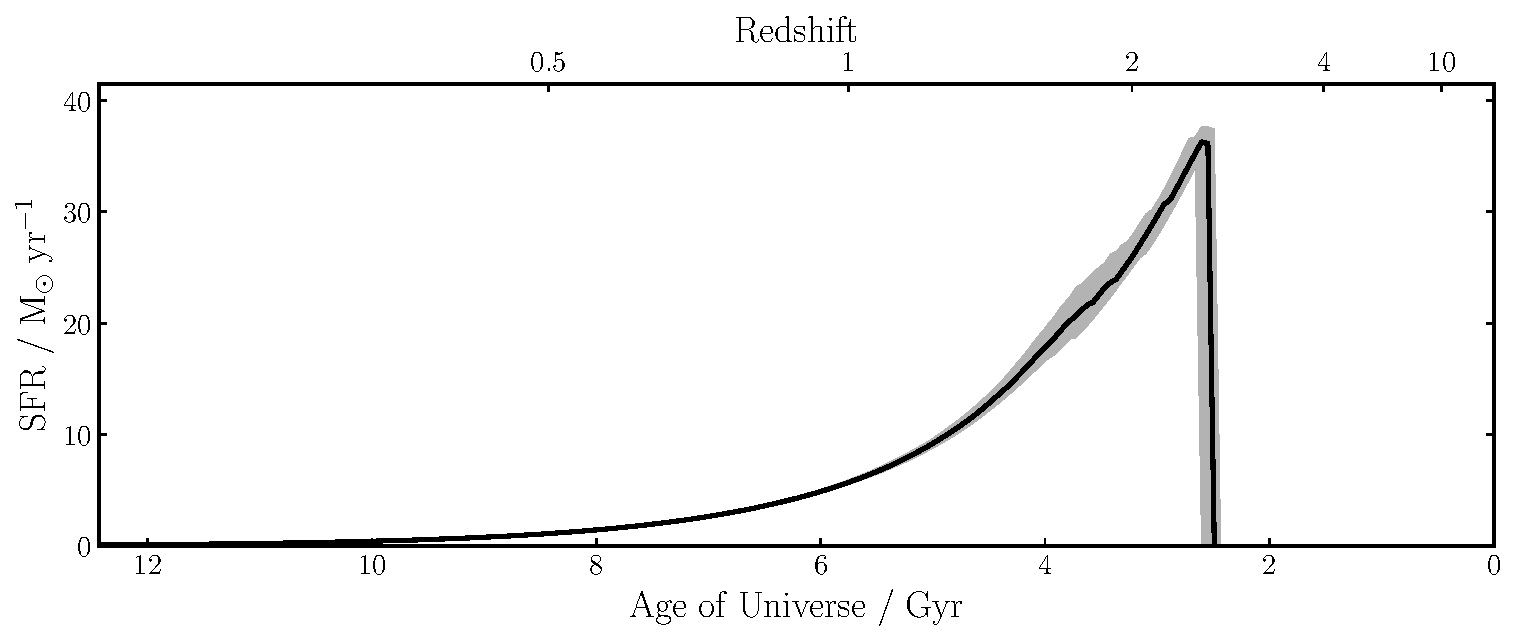
\includegraphics[width=0.9\textwidth]{../pipes/plots/delayed_burst_final/phil_model_7_sfh.pdf}
  \caption{A priori and posterior SFH.}
  \label{}
\end{figure}

\newpage
\begin{figure}[h!]
  \centering
  \includegraphics[width=0.9\textwidth]{../pipes/plots/priors/phil_model_08_sfh.pdf}
  \includegraphics[width=0.9\textwidth]{../pipes/plots/lognormal_burst/phil_model_08_sfh.pdf}
  \includegraphics[width=0.9\textwidth]{../pipes/plots/wide_dblplaw_burst/phil_model_08_sfh.pdf}
  \caption{A priori and posterior SFH.}
  \label{}
\end{figure}

\newpage
\begin{figure}[h!]
  \centering
  \includegraphics[width=0.9\textwidth]{../pipes/plots/priors/phil_model_09_sfh.pdf}
  \includegraphics[width=0.9\textwidth]{../pipes/plots/exponential_burst/phil_model_09_sfh.pdf}
  \includegraphics[width=0.9\textwidth]{../pipes/plots/wide_exponential_burst/phil_model_09_sfh.pdf}
  \caption{A priori and posterior SFH.}
  \label{}
\end{figure}

\newpage
\begin{figure}[h!]
  \centering
  \includegraphics[width=0.9\textwidth]{../pipes/plots/priors/phil_model_10_sfh.pdf}
  \includegraphics[width=0.9\textwidth]{../pipes/plots/exponential_burst/phil_model_10_sfh.pdf}
  \includegraphics[width=0.9\textwidth]{../pipes/plots/wide_dblplaw_burst/phil_model_10_sfh.pdf}
  \caption{A priori and posterior SFH.}
  \label{}
\end{figure}

\end{document}
